In this section, the Link Budget for the Forward Path is computed.

In the first part, the parameters used in the calculation are presented and discussed, then is calculated the Link Budget for the Uplink (\gls{gs} to Satellite), the Downlink (Satellite to the user) and the overall one.
\subsection{Parameters setting and estimation}
	\subsubsection{Antenna Parameters}
		To compute the link budget we need the parameters of Satellite, Ground Station and User antennas. These are taken from \cite{ippolito17} and reported in \autoref{tab:antenna_param}.

		\begin{table}[h]
			\centering
			\begin{tabular}{ccc}
			\toprule
			& Symbol & Value\\
			\midrule
			\gls{gs} antenna diameter (m) & $d_{GS}$ & 6\\
			Sat antenna diameter (m) & $d_{SAT}$  & 1.2\\
			Sat antenna noise temperature (K)& $t_A^{SAT}$ & 290\\
			User antenna diameter (m)& $d_{US}$ & 1\\
			User antenna noise temperature (K)& $t_A^{US}$ & 80\\
			Antennas Efficiency & $\eta$ & 0.6\\
			\bottomrule
			\end{tabular}
			\caption{Antennas parameters used in the Link Budget calculation}
			\label{tab:antenna_param}
		\end{table}

		$t_A^{SAT}$ is set to $290K$ since satellite receiver antenna \textit{sees} the full thermal radiation of the Earth, $t_A^{US}$ is set to $80K$ since typical values for a Ku-Band receiver antenna in the Downlink are between $60K$ and $80K$, and $80K$ is the value that most decrease the Link Budget.
		All the antenna's efficiencies are set to $0.6$, since typical values are between $0.6$ and $0.75$, so the worst case has been taken.

		Knowing the diameter of the antenna reflector, its efficiency and the wavelength of the communication, the gain of each antenna can be computed as in \autoref{eq:gain}.

		\begin{equation}\label{eq:gain}
			g = \eta\bigg(\frac{\pi d}{\lambda}\bigg)^2 \qquad G = 10log\bigg[\eta\bigg(\frac{\pi d}{\lambda}\bigg)^2\bigg] ~dBi
		\end{equation}

		The result for each antenna are in \autoref{tab:antenna_gain}.

		\begin{table}[h]
			\centering
			\begin{tabular}{ccc}
			\toprule
			& Symbol & Value\\
			\midrule
			\gls{gs} antenna gain (dB) & $G_{GS}^{TX}$ & 56.92\\
			Sat antenna gain while receiving (dB) & $G_{SAT}^{RX}$  & 42.94\\
			Sat antenna gain while transmitting (dB) & $G_{SAT}^{TX}$ & 40.68\\
			User antenna gain (dB) & $G_{US}^{RX}$ & 39.1\\
			\bottomrule
			\end{tabular}
			\caption{Gain of each antenna in transmission and reception}
			\label{tab:antenna_gain}
		\end{table}

	\subsubsection{Losses}
		The losses due to noise and attenuation in the payload and some to atmospheric conditions are constant and are reported in \autoref{tab:constant_losses}. All the attenuations are in dB.

		\begin{table}[h]
			\centering
			\begin{tabular}{ccc}
			\toprule
			& Symbol & Value\\
			\midrule
			Input Backoff & $IBO$ & -16\\
			Output Backoff & $OBO$ & -10.47\\
			Losses due to multicarrier operation & $l_{mc}$ & 10.47\\
			Losses due to feeder & $l_{ftx}$  & 0.5\\
			Carrier to interference noise & $C/I$  & 23\\
			Pointing Loss & $l_p$ & 0.3\\
			Gases absorption & $l_{gas}$ & 0.3\\
			\bottomrule
			\end{tabular}
			\caption{Constant losses}
			\label{tab:constant_losses}
		\end{table}
		Losses due to rain $L_{rain}$ and the Path Loss $L_{pl}$ depends on the position of the satellite and on the carrier frequency.

		For the GS we calculated a rain intensity $R = 11.4919  ~mm/h$, we assumed that the rain is 2km high and calculating the rain attenuation as in \autoref{eq:rain_formula} we obtain the plots in \autoref{fig:rain_up} and \autoref{fig:rain_down}.

		\begin{equation}\label{eq:rain_formula}
			L_{rain} = kR^\alpha L_sr_p
		\end{equation}

		\begin{figure}[ht]
			\begin{minipage}{.5\textwidth}
			\centering
			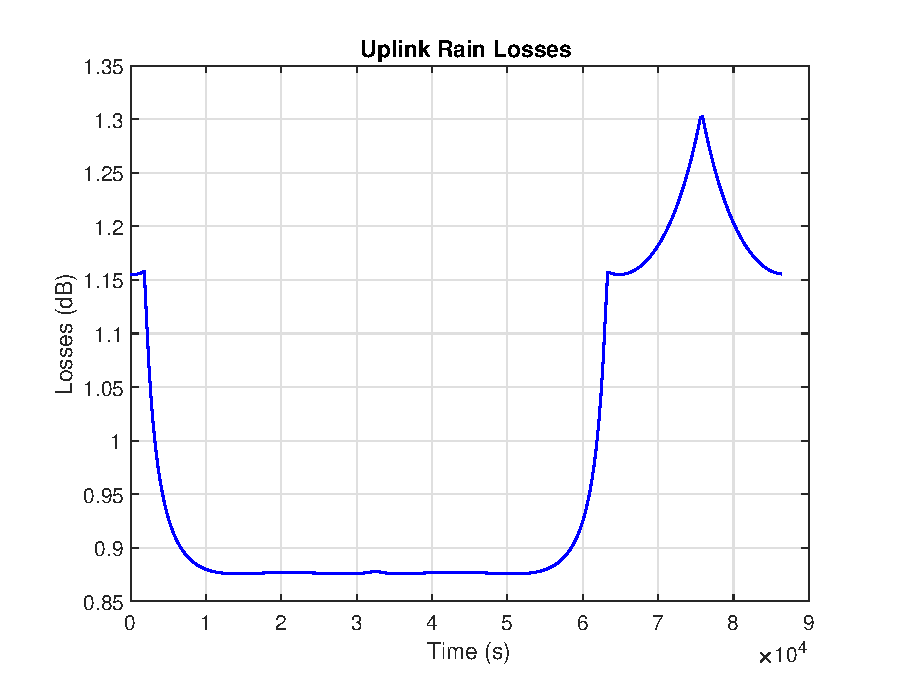
\includegraphics[width = \textwidth]{up_rain.eps}
			\caption{Variation of rain losses in Uplink over the time}
			\label{fig:rain_up}
			\end{minipage}
			\begin{minipage}{.5\textwidth}
			\centering
			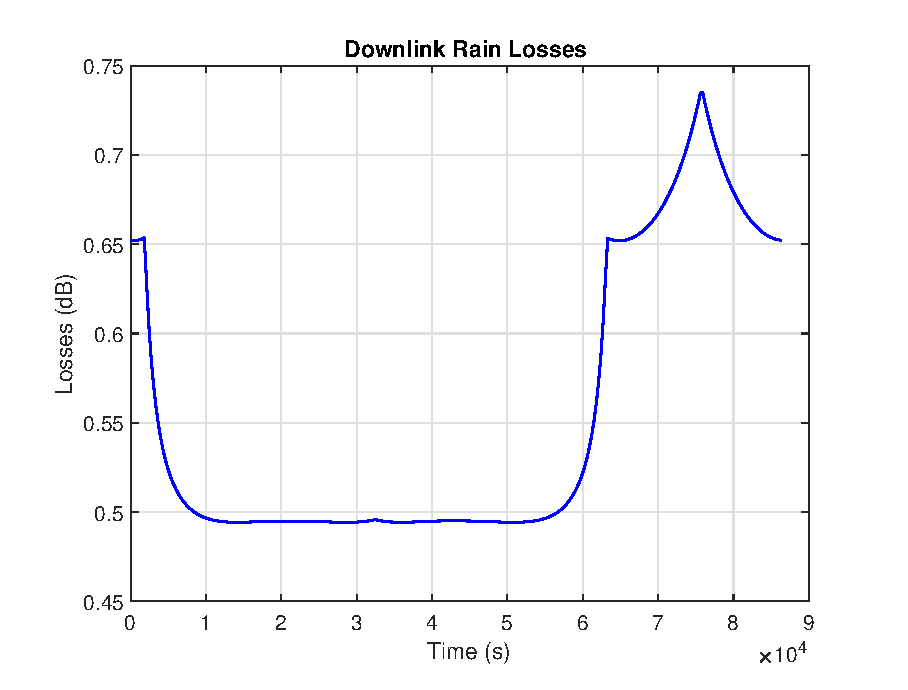
\includegraphics[width = \textwidth]{down_rain.eps}
			\caption{Variation of rain losses in Downlink over the time}
			\label{fig:rain_down}
			\end{minipage}
		\end{figure}

		The parameters in \autoref{eq:rain_formula} are calculated as in \autoref{eq:rain_parameters}.
		\begin{equation}\label{eq:rain_parameters}
			\begin{split}
				k &= 4.21\times 10^{-5}\cdot f^{2.42}\\
				\alpha &= 1.41 \cdot f^{-0-0779}\\
				L_s &= \frac{2km}{sin\theta}\\
				r_p &= \frac{90}{90+4L_scos\theta}
			\end{split}
		\end{equation}
		where $f$ is the carrier frequency in Uplink or in Downlink and $\theta$ is the elevation angle.

		The path loss also depends on the position of the satellite and is calculated with the formula in \autoref{eq:path_loss}, where $r$ is the distance between the satellite and the \gls{gs} or the user, taking in account the altitude of the latter, and $\lambda$ is the wavelength of the communication.

		\begin{equation}\label{eq:path_loss}
			L_{PL} = 20log\bigg(\frac{2\pi r}{\lambda}\bigg) ~dB
		\end{equation}

		Using \autoref{eq:path_loss} in each istant of the simulation, we obtain the plots in \autoref{fig:up_pathloss} and \autoref{fig:down_pathloss}.

		\begin{figure}[ht]
			\begin{minipage}{.5\textwidth}
			\centering
			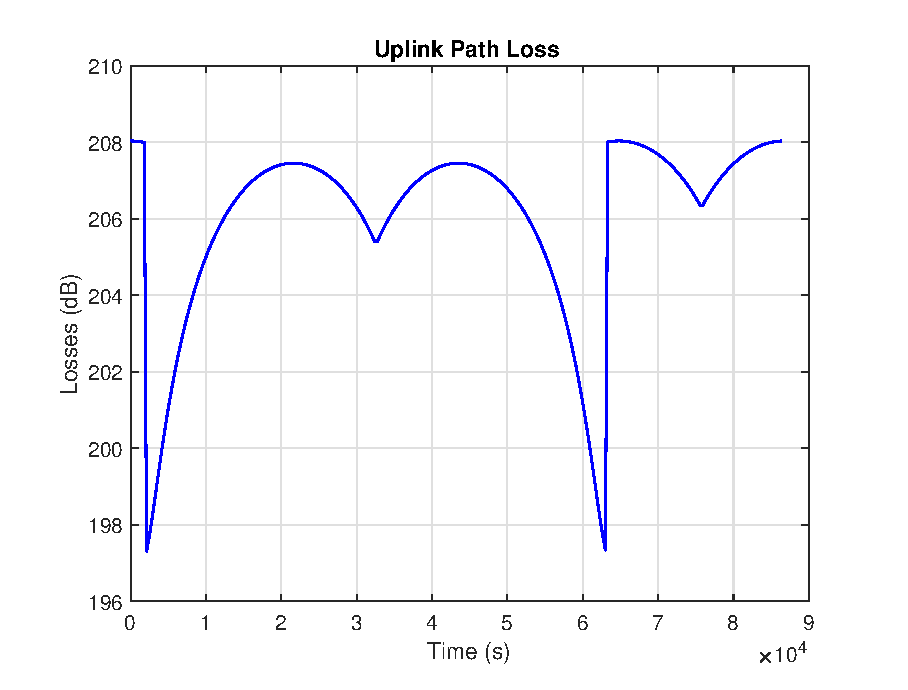
\includegraphics[width = \textwidth]{up_pathloss.eps}
			\caption{Variation of Path Loss in Uplink over the time}
			\label{fig:up_pathloss}
			\end{minipage}
			\begin{minipage}{.5\textwidth}
			\centering
			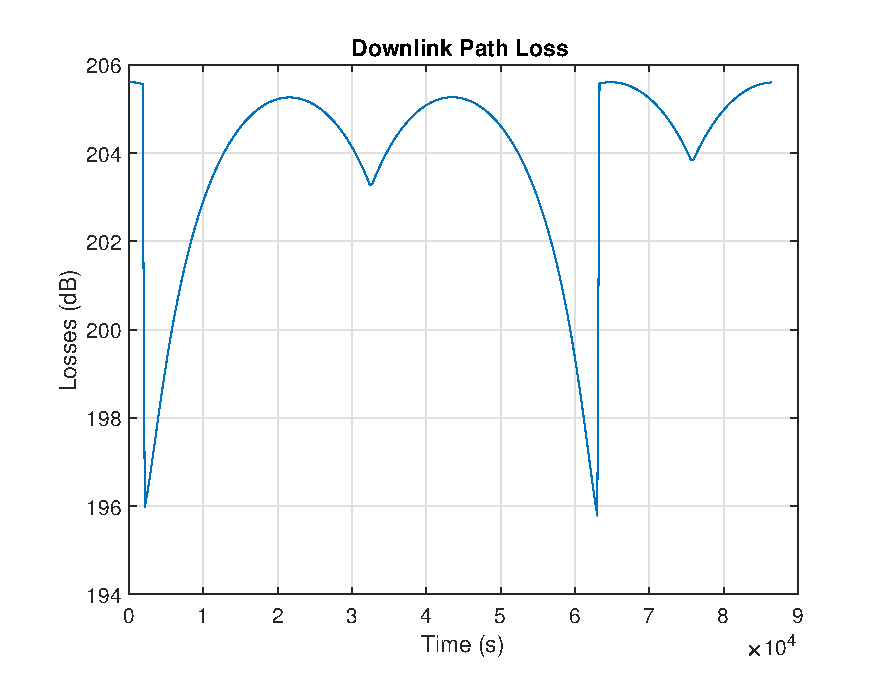
\includegraphics[width = \textwidth]{down_pathloss.eps}
			\caption{Variation of Path Loss in Downlink over the time}
			\label{fig:down_pathloss}
			\end{minipage}
		\end{figure}
	\subsubsection{Effective Isotropic Radiated Power(EIRP)}
	To calculate \gls{eirp} we have to compute firstly the power that each antenna has to transmit $p_{tx}$.
	The power that each transponder has to transmit is calculated as in \autoref{eq:power_1T}, using the parameters yet defined, than this power has to be multiplied for the number of transponder in the system, that in our case is 12, the final formula is in
	\begin{equation}\label{eq:power_1T}
		p_{tx}^{1T} = [p_{HPA}]_{dB} - l_{mc} - l_{ftx}
	\end{equation}
	\begin{equation}\label{eq:power_tot}
		p_{tx} = p_{tx}^{1T} + 10log(12)
	\end{equation}
	Then the \gls{eirp} is calculated for Uplink and Downlink with the formula in \autoref{eq:eirp}.
	\begin{equation}\label{eq:eirp}
		EIRP = G_{tx} + p_{tx}
	\end{equation}
	For the Uplink, using $G_{GS}^{TX}$ as gain, the result is $EIRP_{GS} = 96.79 ~dB$, while for the Downlink, using $G_{SAT}^{TX}$ as gain, the result is $EIRP_{SAT} = 66.58 ~dB$.
\subsection{Uplink}
\subsection{Downlink}
\subsection{Overall Link Budget}
